\documentclass[letterpaper, 10pt]{article} 
%% if A4 paper needed, change letterpaper to A4

\usepackage{opticameet3} %% use version 3 for proper copyright statement

%% provide authormark
\newcommand\authormark[1]{\textsuperscript{#1}}

%% standard packages and arguments should be modified as needed
\usepackage{amsmath,amssymb}
\usepackage[colorlinks=true,bookmarks=false,citecolor=blue,urlcolor=blue]{hyperref} %pdflatex
%\usepackage[breaklinks,colorlinks=true,bookmarks=false,citecolor=blue,urlcolor=blue]{hyperref} %latex w/dvipdf

\begin{document}

\title{Crecimiento de Capital respecto a la variación de tecnología o conocimiento: Modelado con Ecuaciones Diferenciales}

\author{Author name(s)}
% \address{Author affiliation and full address}
% \email{e-mail address}
%%Uncomment the following line to override copyright year from the default current year.
%\copyrightyear{2024}



\author{Jacobo Ruiz David Mauricio,\authormark{1} ~~Ordóñez del Carpio, Jyns Arturo,\authormark{2} ~~and Gutierrez Del Águila, Matías Martin \authormark{2} }

\address{\authormark{1} \href{david.jacobo@utec.edu.pe}{david.jacobo@utec.edu.pe} ~~~~202220396\\
\authormark{2} \\
\authormark{3}
}

\email{\authormark{*}opex@optica.org} %% email address is required 


\begin{abstract}
Este paper propone investigar la relación entre el crecimiento económico y el cambio tecnológico usando ecuaciones diferenciales. Se comparan dos modelos fundamentales, el Modelo Solow-Swan y el Modelo Romer, para analizar cómo el cambio tecnológico influye  en el crecimiento económico a lo largo del tiempo, el analisis matematico se centrará en el primero. El Modelo Solow-Swan se basa en la acumulación de capital físico y tecnología exógena, sugiere que el aumento de productividad solo se explica a través de inversiones directas, crecimiento poblacional y el progreso tecnológico.\cite{Chirwa18} mientras que el Modelo Romer introduce el concepto de crecimiento endógeno, el cual sugiere que el progreso tecnológico ocurre cuando se inventan nuevos productos, y esto a su vez se debe a la investigación y desarrollo (I+D) realizados por empresarios que buscan obtener beneficios económicos \cite{Chu18}. Los objetivos principales de esta investigación son analizar el impacto del cambio tecnológico en el crecimiento económico y modelar la dinámica del crecimiento económico mediante ecuaciones diferenciales.
\end{abstract}

\section*{Keywords}
\begin{flushright}
    Ecuaciones diferenciales, Crecimiento económico, Modelo Solow-Swan, Modelo Romer, Cremiento Exogeno
\end{flushright}

\section*{Objetivos}

\begin{itemize}
  \item Analizar el Impacto del Cambio Tecnológico en el Crecimiento Económico

  \item Modelar la Dinámica del Crecimiento Económico mediante Ecuaciones Diferenciales
\end{itemize}

\section{Introducción}

El crecimiento económico es un tema fundamental en la economía que se ha estudiado durante décadas. El crecimiento económico se define como el aumento de la producción de bienes y servicios en una economía en un período de tiempo determinado. La mayoría de los economistas están de acuerdo en que el crecimiento económico es un factor fundamental para mejorar el bienestar de la sociedad, ya que permite a las personas consumir más bienes y servicios. \cite{Moret09} El crecimiento económico se mide mediante el Producto Interno Bruto (PIB) y el Producto Interno Bruto per cápita (PIB per cápita), que es el PIB dividido por la población total. El PIB per cápita se utiliza para comparar el nivel de vida entre diferentes países. El crecimiento económico se puede lograr aumentando la cantidad de factores de producción, como la fuerza laboral y el capital físico, y mejorando la eficiencia de los factores de producción, como el progreso tecnológico. \cite{Moret09}

%% TO-DO


\section{Marco Teorico}
  Para comprender este documento es necesario comprender los conceptos clave y los modelos fundamentales que se utilizarán como base para el análisis. A continuación, se definen de manera sencilla los conceptos y modelos clave:


  
\begin{enumerate}

  
  \item \textbf{Crecimiento Económico}: El crecimiento económico segun lo define Patricia Castillo Marin \cite{Eco11}:
  
    \begin{quote}
      \text{" [...]} \textit{ se define como el proceso en virtud del cual la renta real per cápita de un país aumenta durante un largo período de tiempo. En otros términos, el desarrollo es un proceso integral, socioeconómico, que implica la expansión continua del potencial económico}
    \end{quote}
    Para entender el crecimiento económico, es crucial analizar las fuentes que lo impulsan, en particular, la acumulación de capital y el cambio tecnológico.

  \item \textbf{Cambio Tecnológico}: El cambio tecnológico se refiere a la mejora y avance de los métodos y procesos de producción, así como a la creación de nuevos productos y tecnologías. Este factor es fundamental para los modelos de crecimiento exógeno como el de Solow-Swan\cite{Chirwa18}.
  
  \item \textbf{Modelos de Crecimiento Económico}: Para analizar el crecimiento económico respecto a variables principalmente economicas y policitas hay dos modelos que han tenido una mayor extensión en el ambito academico: el Modelo Solow-Swan y su predecesor, el Modelo Romer.
  
  \begin{itemize}
     
    \item \textbf{Modelo Solow-Swan}: Este modelo, propuesto por Robert Solow y Trevor Swan en la década de 1950, se basa en la acumulación de capital físico, el crecimiento de la fuerza laboral y el progreso tecnológico como motores del crecimiento económico.\cite{Martin11} 
    En este enfoque, la tecnología se considera exógena, lo que significa que no se modifica internamente en la economía, sino que se toma como un factor dado. Otra interpretación del desarrollo tecnologico como factor exógeno, segun Chirwa \cite{Chirwa18} es que el desarrollo tecnologico es el factor de mayor importancia en el crecimiento economico a largo plazo.
  
    \item \textbf{Modelo Romer}: El Modelo Romer, desarrollado por Paul Romer en la década de 1980, introduce el concepto de crecimiento endógeno. En contraste con el Modelo Solow-Swan, sugiere que el progreso tecnológico es influenciado por las acciones de las empresas que buscan obtener ganancias a través de la investigación y el desarrollo (I+D)\cite{Casparri13} . Este modelo considera que el conocimiento y la tecnología pueden ser impulsados por políticas gubernamentales y la inversión en I+D.
  
  \end{itemize}

  \item \textbf{Ecuaciones Diferenciales en Economía}: Las ecuaciones diferenciales son herramientas matemáticas ampliamente utilizadas en la economía para modelar y analizar sistemas dinámicos en los que las variables cambian con respecto al tiempo. Estas ecuaciones permiten describir cómo evolucionan ciertas magnitudes económicas en función de diversas variables, lo que resulta esencial en la comprensión de fenómenos económicos complejos.

\end{enumerate}

\section{Modelo Matematico}

Acontinuación se presenta ambos modelos matematicos en su forma de ecuaciones diferenciales, así como una breve explicación de cada una de ellas, junto con sus variables y parametros de los que dependen.

\subsection{Modelo Solow-Swan}

El modelo Solow-Swan se basa en la acumulación de capital físico y tecnología exógena, sugiere que el aumento de productividad solo se explica a través de inversiones directas, crecimiento poblacional y el progreso tecnológico.\cite{Chirwa18} El modelo Solow-Swan se puede representar mediante la siguiente ecuación diferencial:

\begin{equation}
  \frac{dK}{dt} = sY - \delta K
\end{equation}

Donde:

\begin{itemize}
  \item $K$ es el capital físico
  \item $Y$ es el producto
  \item $s$ es la tasa de ahorro
  \item $\delta$ es la tasa de depreciación
  
\end{itemize}

\subsection{Modelo Romer}

El Modelo Romer, desarrollado por Paul Romer en la década de 1980, introduce el concepto de crecimiento endógeno. En contraste con el Modelo Solow-Swan, sugiere que el progreso tecnológico es influenciado por las acciones de las empresas que buscan obtener ganancias a través de la investigación y el desarrollo (I+D)\cite{Casparri13} . Este modelo considera que el conocimiento y la tecnología pueden ser impulsados por políticas gubernamentales y la inversión en I+D. El modelo Romer se puede representar mediante la siguiente ecuación diferencial:


Figures and illustrations should be incorporated directly into the
manuscript, and the size of a figure should be commensurate with the amount
and value of the information conveyed by the figure.

\begin{figure}[htbp]
  \centering
  %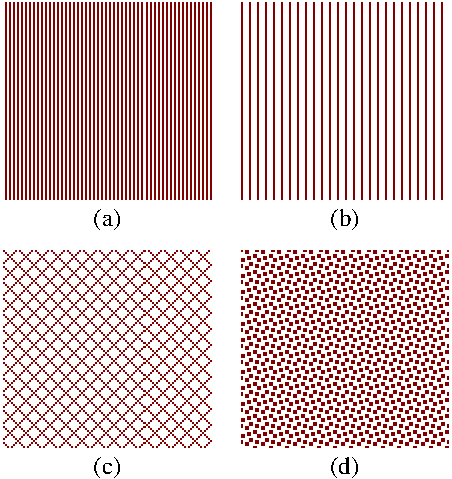
\includegraphics[width=8.3cm]{OT10000F1}
\caption{Sample figure with preferred style for labeling parts.}
\end{figure}


\begin{table}[htb]
 \centering \caption{Sample Table}
\begin{tabular}{ccc}
    \hline
    One & Two & Three \\
    \hline
    Eins & Zwei & Drei \\
    Un & Deux & Trois \\
    Jeden & Dv\v{e} & T\v{r}i \\
    \hline
   \end{tabular}
    \end{table}

No more than three figures should generally be included in the paper. Place figures as close as possible to where they
are mentioned in the text. No part of a figure should extend beyond text width, and text should not wrap around figures. Please provide permission and attribution for any trademarked or copyright images.

\section{References}
References should be cited with the \verb+\cite{}+ command.
Bracketed citation style, as opposed to superscript, is preferred
\cite{Chirwa18,Chu18,masters93, , , , }.
The \texttt{opticameet3.sty} style file references \texttt{cite.sty}. Comprehensive journal abbreviations are available on the Crossref web site:
\href{http://www.crossref.org/titleList/}{http://www.crossref.org/titleList/}.



\begin{thebibliography}{99} %% use BibTeX or add references manually



\bibitem{Chirwa18}Chirwa, T. G., \& Odhiambo, N. M. (2018). Exogenous and endogenous growth models: A critical review. Comparative Economic Research. Central and Eastern Europe, 21(4), 63-84.\\
\url{https://www.econstor.eu/handle/10419/259181}.

\bibitem{Chu18}Chu, A. C. (2018). From Solow to Romer: Teaching endogenous technological change in undergraduate economics. International Review of Economics Education, 27, 10-15.

\bibitem{Eco11}Económico, D. E. S. A. R. R. O. L. L. O. (2011). Política económica: crecimiento económico, desarrollo económico, desarrollo sostenible. Revista internacional del mundo económico y del derecho, 3, 1-12.

\bibitem{Moret09} Morettini, M. (2009). El modelo de crecimiento de Solow.

\bibitem{Martin11} Martín, M. Á. G. (2011). Crecimiento económico. ICE, Revista de Economía, (858).
\bibitem{Casparri13} Casparri, M. T. (2013). Un modelo dinámico de crecimiento endógeno (Doctoral dissertation, Facultad de Ciencias Económicas. Universidad de Buenos Aires).

\end{thebibliography}

\end{document}
